\documentclass[11pt]{article}  % need to compile twice
\usepackage{amsmath, textcomp, amssymb, geometry, graphicx, enumerate, ctex, xcolor, float}
\usepackage[colorlinks, linkcolor=black]{hyperref}
\usepackage{listings}		% 为了避免与页眉的兼容问题可将listings放入table环境中
\lstset{
    basicstyle          =   \sffamily,          % 基本代码风格
    keywordstyle        =   \color{blue},          % 关键字风格
    keywordstyle    =   [2] \color{teal},
    commentstyle        =   \rmfamily\itshape,  % 注释的风格,斜体
    stringstyle         =   \ttfamily,  % 字符串风格
    flexiblecolumns,                % 别问为什么,加上这个
    numbers             =   left,   % 行号的位置在左边
    showspaces          =   false,  % 是否显示空格,显示了有点乱,所以不现实了
    numberstyle         =   \zihao{-5}\ttfamily,    % 行号的样式,小五号,tt等宽字体
    showstringspaces    =   false,
    captionpos          =   t,      % 这段代码的名字所呈现的位置,t指的是top上面
    frame               =   lrtb,   % 显示边框
    basicstyle          =   \zihao{-5}\ttfamily,
    stringstyle         =   \color{magenta},
    commentstyle        =   \color{red}\ttfamily,
    breaklines          =   true,   % 自动换行,建议不要写太长的行
    columns             =   fixed,  % 如果不加这一句,字间距就不固定,很丑,必须加
    basewidth           =   0.5em,
}
\geometry{left=2.54cm, right=2.54cm, top=3.18cm, bottom=3.18cm}

\def\Name{杨豪\space}  % Your name
\def\SID{2206213297}  % Your student ID number

% need to be confirmed before each time writing and committing 
\def\Homework{2} % Number of Homework
\def\Session{2022-Fall}
\def\CourseCodeName{SOFT500327: 算法设计与分析}
\def\simCourseName{Algo}

\title{\vspace{-4cm}\CourseCodeName \space
        \Session \protect\\  Homework-\textbf{\Homework} Solutions}
\author{软件2101 \Name \space 学号: \SID}
\markright{\simCourseName\ \space \Session\  HW-\Homework\ \Name}
\date{\today}

\begin{document}
\maketitle

\textbf{Honor Code: I promise that I finished the homework solutions on my own without copying other people's 
    work.}

pdf中所示源码均附于src/文件夹中

\section*{3-2}

\subsection*{代码}

    \begin{figure}[H]
        \centering
        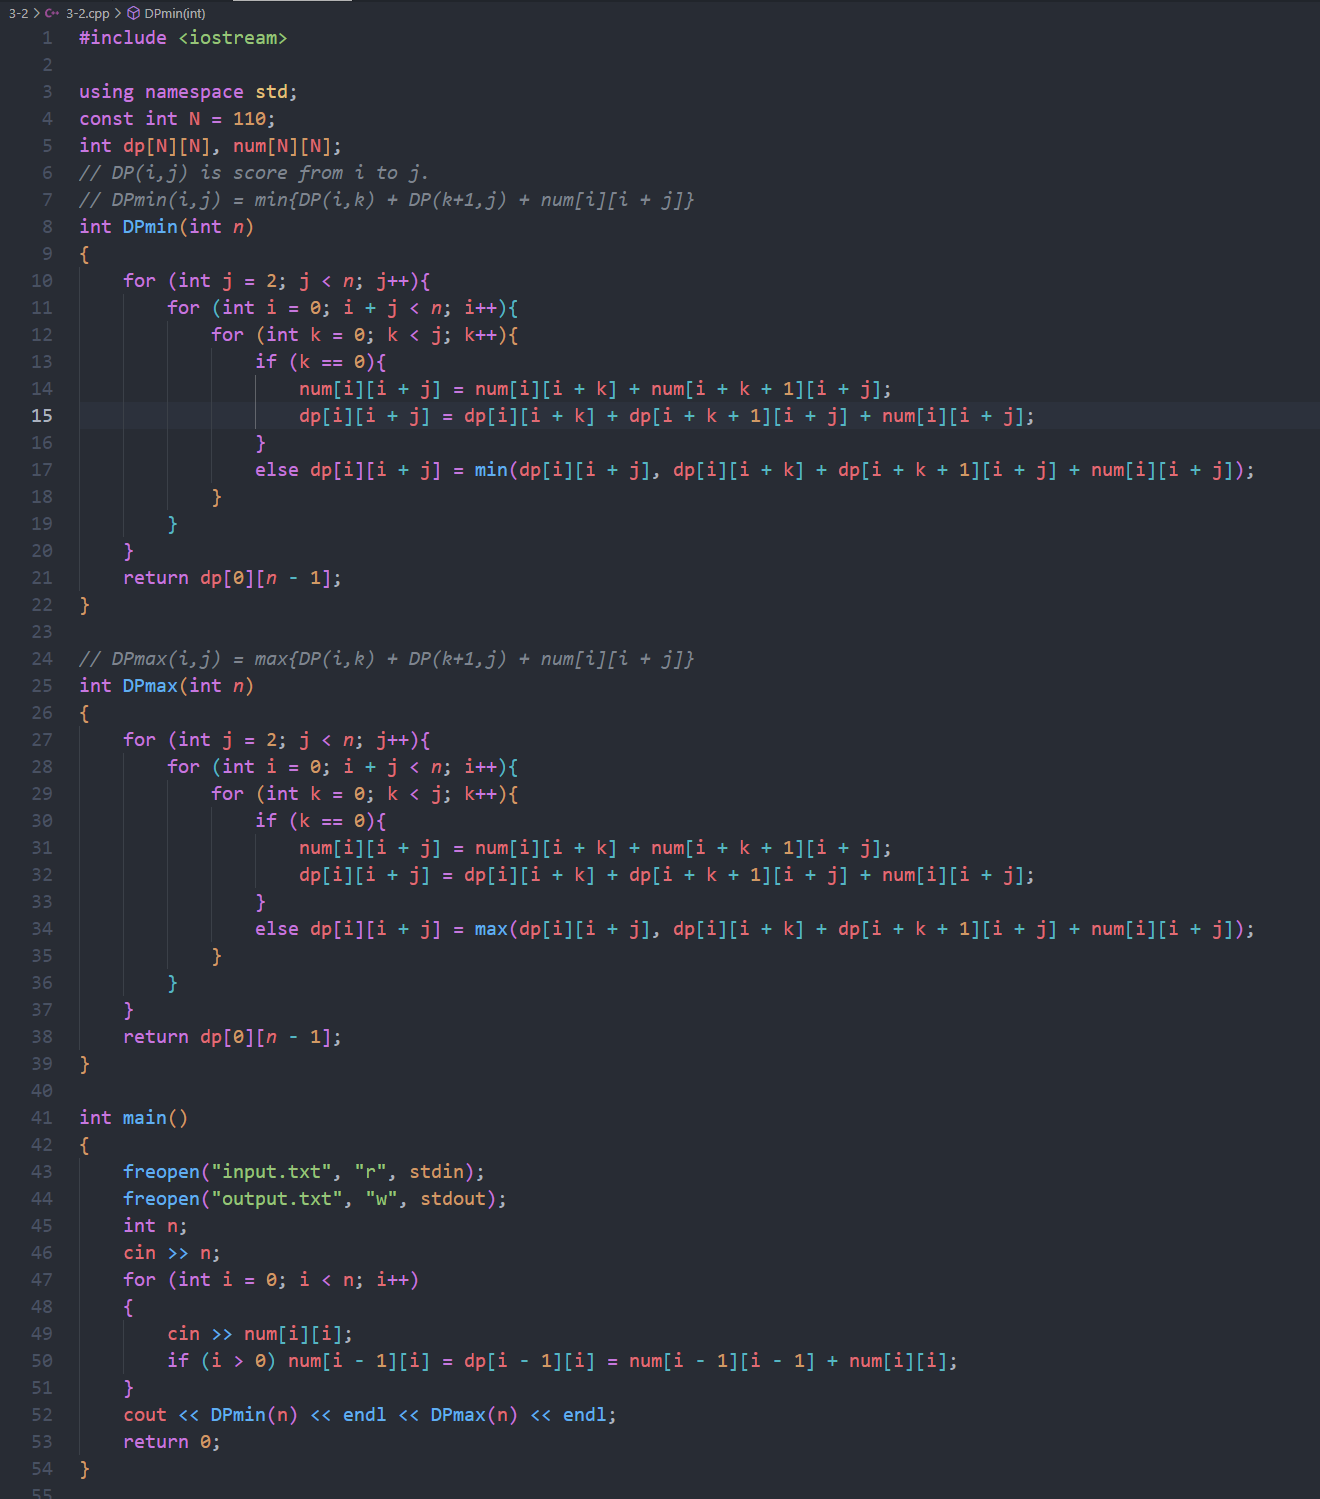
\includegraphics[width = 0.8\textwidth]{pic/3-2.png}
    \end{figure}

\subsection*{输入}

    \begin{figure}[H]
        \centering
        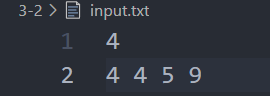
\includegraphics[width = 0.3\textwidth]{pic/3-2in.png}
    \end{figure}

\subsection*{输出}

    \begin{figure}[H]
        \centering
        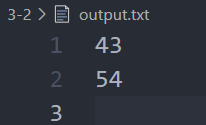
\includegraphics[width = 0.3\textwidth]{pic/3-2out.png}
    \end{figure}

\section*{3-4}

\subsection*{代码}

    \begin{figure}[H]
        \centering
        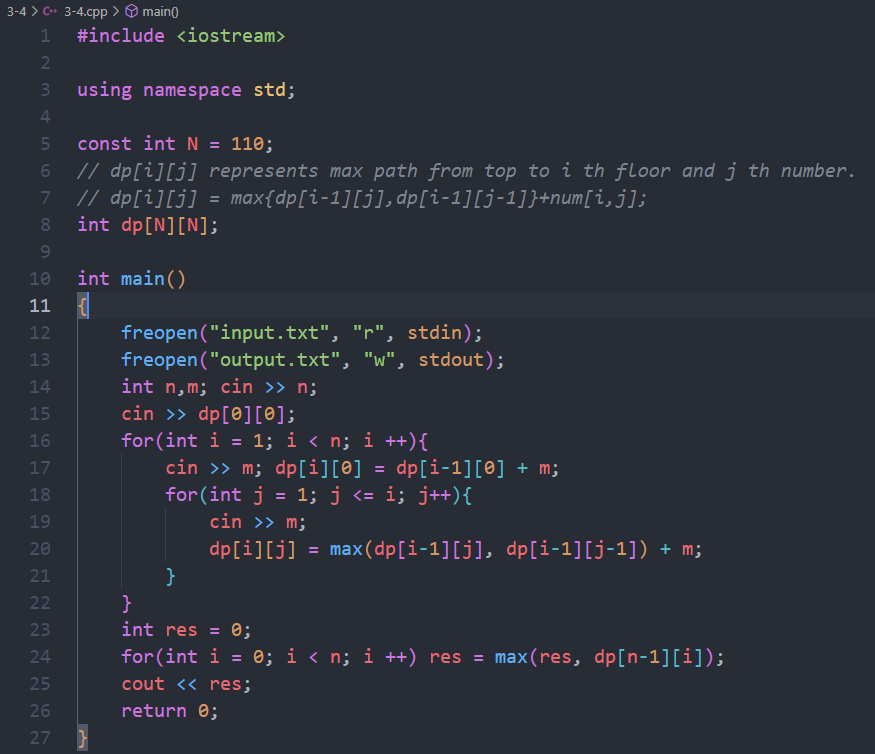
\includegraphics[width = 0.8\textwidth]{pic/3-4.png}
    \end{figure}

\subsection*{输入}

    \begin{figure}[H]
        \centering
        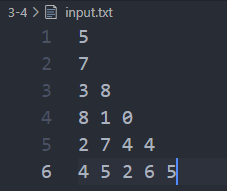
\includegraphics[width = 0.3\textwidth]{pic/3-4in.png}
    \end{figure}

\subsection*{输出}

    \begin{figure}[H]
        \centering
        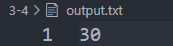
\includegraphics[width = 0.3\textwidth]{pic/3-4out.png}
    \end{figure}

\section*{3-6}

\subsection*{代码}

    \begin{figure}[H]
        \centering
        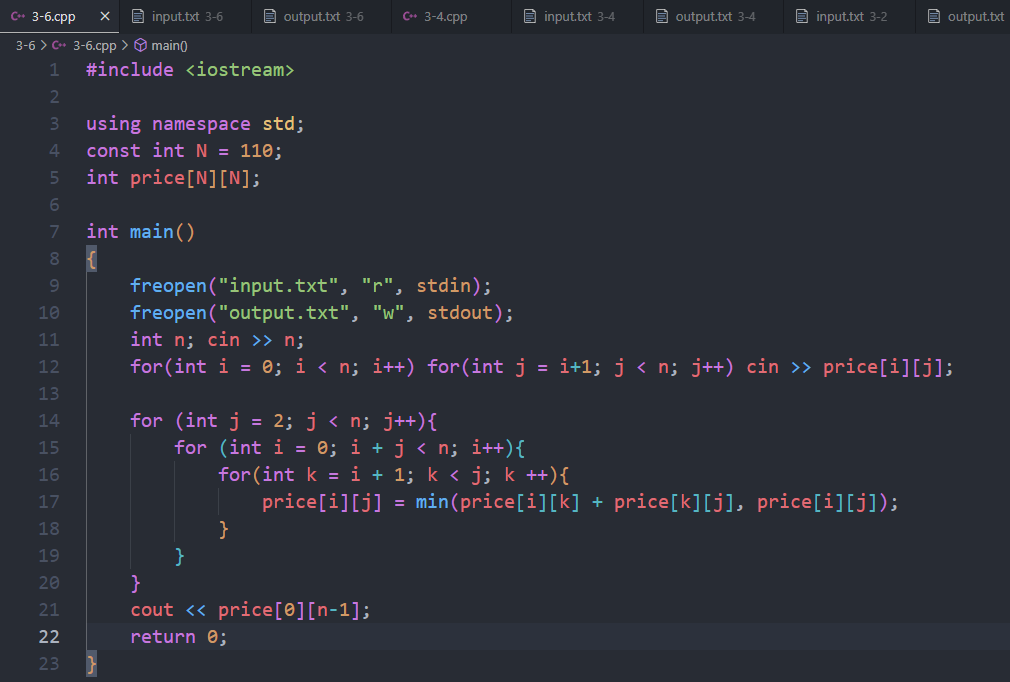
\includegraphics[width = 0.8\textwidth]{pic/3-6.png}
    \end{figure}

\subsection*{输入}

    \begin{figure}[H]
        \centering
        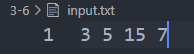
\includegraphics[width = 0.3\textwidth]{pic/3-6in.png}
    \end{figure}

\subsection*{输出}

    \begin{figure}[H]
        \centering
        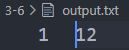
\includegraphics[width = 0.3\textwidth]{pic/3-6out.png}
    \end{figure}

\section*{4-1}

\subsection*{代码}

    \begin{figure}[H]
        \centering
        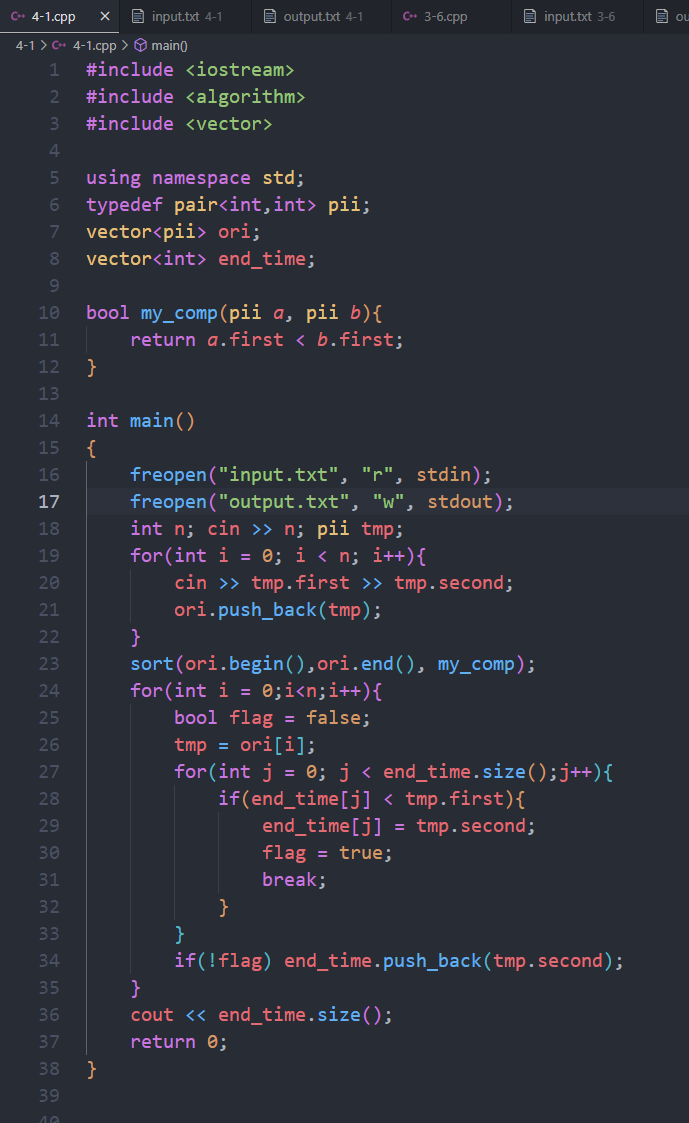
\includegraphics[width = 0.8\textwidth]{pic/4-1.png}
    \end{figure}

\subsection*{输入}

    \begin{figure}[H]
        \centering
        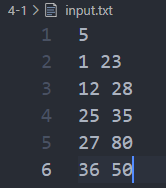
\includegraphics[width = 0.3\textwidth]{pic/4-1in.png}
    \end{figure}

\subsection*{输出}

    \begin{figure}[H]
        \centering
        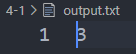
\includegraphics[width = 0.3\textwidth]{pic/4-1out.png}
    \end{figure}

\section*{4-9}

\subsection*{证明}

对于选好的分割
如果还有更小值,则需要将其中n组相邻合为$n_1$个。将每相邻分割的分界线看做一个边。
这里看做是对已选定的边进行“平移”,直接去掉某条边看做该边平移至下一条边。显然,每次平移至少需要一条边向后平移。

假设可以平移,则对于向后平移的边,其平移所得到的 新分割之和 ≥ 原分割之和 + 原边所在的下一个数
且要求 新分割之和<n,但如果新分割之和<n,原边就并不符合我们贪心的算法。


\subsection*{代码}

    \begin{figure}[H]
        \centering
        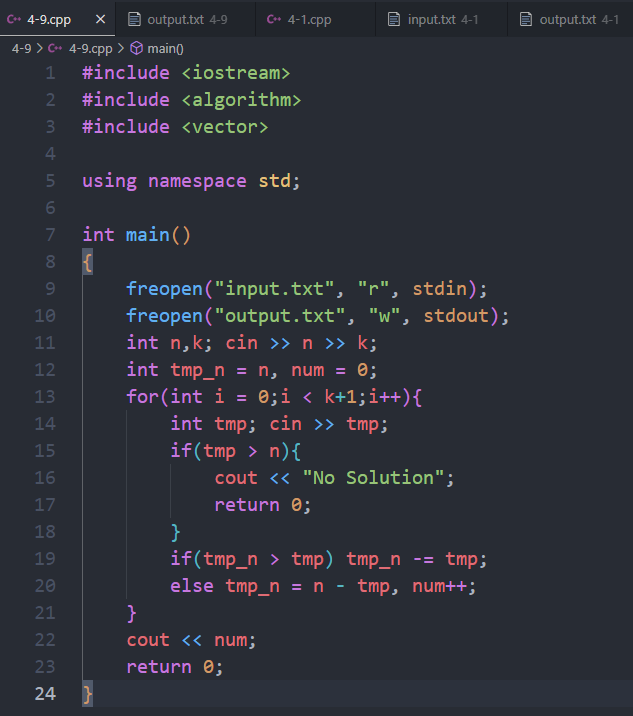
\includegraphics[width = 0.8\textwidth]{pic/4-9.png}
    \end{figure}

\subsection*{输入}

    \begin{figure}[H]
        \centering
        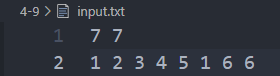
\includegraphics[width = 0.3\textwidth]{pic/4-9in.png}
    \end{figure}

\subsection*{输出}

    \begin{figure}[H]
        \centering
        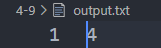
\includegraphics[width = 0.3\textwidth]{pic/4-9out.png}
    \end{figure}

\section*{4-11}

\subsection*{代码}

    \begin{figure}[H]
        \centering
        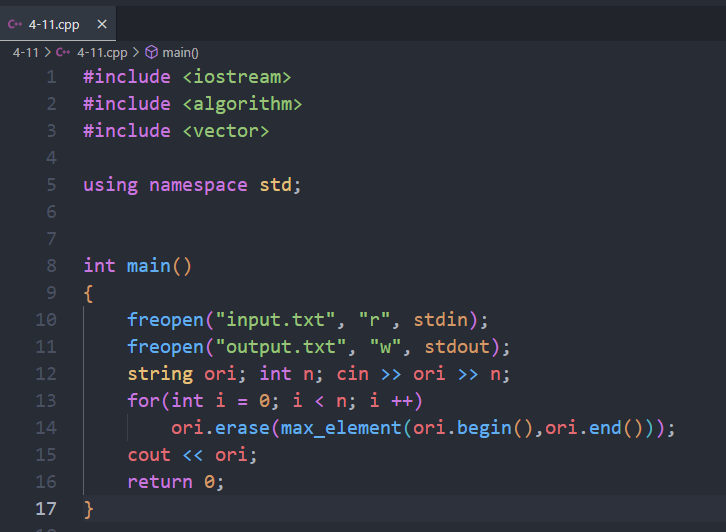
\includegraphics[width = 0.8\textwidth]{pic/4-11.png}
    \end{figure}

\subsection*{输入}

    \begin{figure}[H]
        \centering
        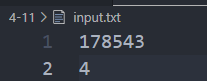
\includegraphics[width = 0.3\textwidth]{pic/4-11in.png}
    \end{figure}

\subsection*{输出}

    \begin{figure}[H]
        \centering
        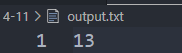
\includegraphics[width = 0.3\textwidth]{pic/4-11out.png}
    \end{figure}
    

\section*{Other things}

\LaTeX \space code refer to these things and was complied on texlive2020.
\begin{itemize}
    \item  \href{https://www.eecs70.org/assets/misc/homework_template.tex}{UCB-CS70's given homework template.} 
    \item  \href{https://www.latexlive.com}{A free website useful to edit \LaTeX \space formula code.}
\end{itemize}

Thanks for your correcting and grading :).

\end{document}

 
